\documentclass{article}
%color definitions
% \definecolor{ashgrey}{rgb}{0.7, 0.75, 0.71}
% \definecolor{bondiblue}{rgb}{0.0, 0.58, 0.71}
% \definecolor{blue(ryb)}{rgb}{0.01, 0.28, 1.0}
% \definecolor{byzantium}{rgb}{0.44, 0.16, 0.39} %morado
% \definecolor{darkgreen}{rgb}{0.0, 0.2, 0.13}
% \definecolor{darkspringgreen}{rgb}{0.09, 0.45, 0.27}
% \definecolor{dartmouthgreen}{rgb}{0.05, 0.5, 0.06}
% \definecolor{debianred}{rgb}{0.84, 0.04, 0.33}
% \definecolor{mygray}{rgb}{0.5,0.5,0.5}
% \definecolor{aurometalsaurus}{rgb}{0.43, 0.5, 0.5}
% \definecolor{asparagus}{rgb}{0.53, 0.66, 0.42}
% \definecolor{arylideyellow}{rgb}{0.91, 0.84, 0.42}
% \definecolor{brown(traditional)}{rgb}{0.59, 0.29, 0.0}
% \definecolor{brass}{rgb}{0.71, 0.65, 0.26}
% \definecolor{carrotorange}{rgb}{0.93, 0.57, 0.13}
% \definecolor{darkpastelblue}{rgb}{0.47, 0.62, 0.8}
% \definecolor{brandeisblue}{rgb}{0.0, 0.44, 1.0}

\usepackage[utf8]{inputenc}
\usepackage[binary-units]{siunitx}
\usepackage[shortcuts]{extdash}
\usepackage[margin=1.5cm]{geometry}
\usepackage[table,xcdraw]{xcolor}
\usepackage[printonlyused]{acronym} %for acronyms
\usepackage{hyperref} %para url
\hypersetup{
    colorlinks=true,
    linkcolor=blue,
    filecolor=magenta,      
    urlcolor=brandeisblue,
}
\usepackage{mathtools} % loads amsmath
\usepackage{textcomp} %\textregistered % or \textcopyright
\usepackage{soul} % para tachar texto con una linea e.g \st{texto tachado}
\usepackage{colortbl}
\usepackage{multicol}
\usepackage{multirow}
\usepackage{makecell}
\usepackage{hhline}
\usepackage{array}
\usepackage{graphicx}
\usepackage{caption}
\usepackage{lscape}
\usepackage{afterpage}
\usepackage{pgf}
\usepackage{cleveref} %for references
%music packages
\usepackage{musicography}
\usepackage{stackengine}
%%para escribir codigo en LaTeX
\usepackage{soul} %% to enable highlight a una linea de codigo
\usepackage{listings,lstautogobble}[showlines=htrue,breakatwhitespace=true] 
\lstloadlanguages{C}
\lstset{ %language=[Sharp]C, %necesario para el emphasize,
basicstyle=\fontfamily{pcr}\selectfont\footnotesize\color{black},
keywordstyle=\color{blue(ryb)}\bfseries, % style for keywords
commentstyle=\color{dartmouthgreen}\ttfamily,
stringstyle=\color{brown(traditional)}\ttfamily, %procnamestyle=\color{brown(traditional)}\ttfamily
%morecomment=[l][\color{brass}]{\#include},
%morecomment=[l][\color{brass}]{\#define},
%morecomment=[s][\color{brown(traditional)}]{/´}{´},
morecomment=*[l][\special@on\color{dartmouthgreen}\itshape]{//},
morecomment=*[s][\special@on\color{dartmouthgreen}\itshape]{/*}{*/},
%morecomment=*[n][\special@on\color{darkpastelblue}]{(0x}{x0)},
morestring=*[b][\special@on\color{byzantium}]",
%escapechar=|,%
otherkeywords={!,!=,~,\$,<, >=,=<,\_t,\_32},
morekeywords={char,
const,
bool,
double,
float,
int,
int8,
int16,
int32,
long,
List,
sizeof,
short,
static,
struct,
typedef,
union,
BaseType,
Queue,
QueuePointers,
SemaphoreData,
TaskHandle,
TaskFunction,
TickType,
TimerHandle,
UBaseType,
uint,
uint8,
uint16,
uint32,
uint64,
unsigned,
volatile, 
void,
xQUEUE},
escapeinside={(*@}{@*)},
numbers=left, % where to put the line-numbers
breaklines=true, %para hacer wrap lines
numberstyle=\small, % the size of the fonts that are used for the line-numbers     
backgroundcolor=\color{white},
tabsize=2,
showspaces=false, % show spaces adding particular underscores
showstringspaces=false, % underline spaces within strings
showtabs=false,
alsoletter={_,\#,*},
emph={\#if, \#include, \#define, \#else, \#endif,\#ifdef,\#ifndef},
emphstyle={[2]\color{blue}},
emphstyle=\color{darkscarlet},
 emph={[2]
 timInfo,
 timer_alarm,
 timer_autoreload,
 timer_config,
 timer_count_dir,
 timer_group,
 timer_idx,
 timer_intr_mode,
 timer_isr,
 timer_start,
 timer_src_clk,
 gpio_num
},
literate={./}{
{{\color{red}./}}}2 
{.^}{{{\color{red}.\^{}}}}2 {&&}{{{\color{red}\&\&{}}}}2 %{=}{{{\color{red}=}}}1 {.}{{{\color{debianred}.}}}1 {!}{{{\color{red}!}}}1
{Ä}{{\"A}}1%
{Ö}{{\"O}}1%
{Ü}{{\"U}}1%
{ä}{{\"a}}1%
{ö}{{\"o}}1%
{ü}{{\"u}}1
{á}{{\'a}}1
{é}{{\'e}}1
{í}{{\'i}}1
{ó}{{\'o}}1
{ú}{{\'u}}1
{ñ}{{\~{n}}}1 % ñ = alt + 164
%{_}{{\_}}1
{^}{{\^{}}}1
{~}{{$\sim$}}1
{orOPER}{{||}}1
{orEqual}{{|=\,\,\,}}1
{&=}{{\&=\,\,\,}}1
%{>}{{$>$\,\,\,}}1
{<}{{$<$\,\,\,}}1
{resHochkomma}{{\textbackslash"}}1
{==}{{$==$\,\,}}1%
{equal=}{{$=$\,\,}}1%
{\%}{{\%\,\,}}1%
{e=}{{$=$\,\,\,}}1
{ß}{{\ss}}1%
{ç}{{\c{c}}}1,
framexrightmargin=5mm, 
frame=shadowbox, 
rulesepcolor=\color{bondiblue},
autogobble=true}
\usepackage{filecontents} %create data datatable
\usepackage{pgfplots}
\pgfplotsset{compat=1.16}
\usepgfplotslibrary{units}
\usepackage{forloop}
%\usepackage{fmtcount}

%for good fracs numbers visualization in tables
\newcolumntype{C}{>{$}c<{$}}



% normal line of code
% highlighted line of code
% lighter blue highlight
% darker blue highlight 

%%%%%%%%%%%%%%%%%%%%%%%%%%%%%%%%%%%%%%%%%%%%%%%%%%%%%%%%%%%%%%%%%%%%%%%%%%%%%%

\newcommand\realnumberstyle[1]{}

\makeatletter
\newcommand{\zebra}[3]{%
    {\realnumberstyle{#3}}%
    \begingroup
    \lst@basicstyle
    \ifodd\value{lstnumber}%
        \color{#1}%
    \else
        \color{#2}%
    \fi
        \rlap{\hspace*{\lst@numbersep}%
        \color@block{\linewidth}{\ht\strutbox}{\dp\strutbox}%
        }%
    \endgroup
}
\makeatother

%Tikz package
\usepackage{tikz}
\usepackage{verbatim}




% Style to select only points from #1 to #2 (inclusive)
\makeatletter

\newif\ifspecial@env@
\def\special@on{\global\special@env@true}
\def\special@off{\global\special@env@false}

\lst@AddToHook{DetectKeywords}{%
    \global\let\last@lst@thestyle=\lst@thestyle
}

\def\emphstyle{%
    \last@lst@thestyle
    \aftergroup\special@off
    \underbar
}

\def\keywordstyle{%
    \ifspecial@env@
        \last@lst@thestyle
    \else
        \color{blue}%
    \fi
    \aftergroup\special@off
}
\makeatother


%\usepackage[active]{preview}
%\PreviewEnvironment{tikzpicture}
\usetikzlibrary{shapes,arrows,chains}
%\setlength\PreviewBorder{5mm}%
%FLOW CHART COMMAND

%pagina en blanco
\newcommand\blankpage{%
    \null
    \thispagestyle{empty}%
    \addtocounter{page}{-1}%
    \newpage}
    
%% HERE SOME TEXT SCPAPES
\newcommand{\BASEPRI}{\texttt{BASEPRI }}
\newcommand{\FIFO}{\texttt{FIFO }}
\newcommand{\IO}{\texttt{I/O }}
\newcommand{\idle}{\texttt{idle }}
\newcommand{\ISR}{\texttt{ISR }}
\newcommand{\IPSR}{\texttt{IPSR }}
\newcommand{\IRQ}{\texttt{IRQ }}
\newcommand{\ICR}{\texttt{ICR }}
\newcommand{\mailbox}{\texttt{mailbox }}
\newcommand{\NVIC}{\texttt{NVIC }}
\newcommand{\PRIMASK}{\texttt{PRIMASK }}
\newcommand{\RAM}{\texttt{RAM }}
\newcommand{\register}{\texttt{register }}
\newcommand{\ROM}{\texttt{ROM }}
\newcommand{\SysTick}{\texttt{SysTick }}
\newcommand{\TExaS}{\texttt{TExaS }}
\newcommand{\UART}{\texttt{UART }}



%new custom commads, defined by Kike.
\newcommand{\ADCbit}[1]{\texttt{ADC{#1}}}
\newcommand{\ADCREG}[1]{\texttt{ADC\_{#1}\_R}}
\newcommand{\bitsRange}[2][50]{\texttt{{#1}-{#2}}}
\newcommand{\CustomHex}[2][0000]{\texttt{0x{#1}.{#2}}}
\newcommand{\GPIOPort}[1]{\texttt{GPIO\_PORT{#1}}}
\newcommand{\GPIOPortR}[2][A]{\texttt{GPIO\_PORT{#1}\_{#2}\_R}}
\newcommand{\GPIOPortHandler}[1]{\texttt{GPIO\_PORT{#1}\_Handler}}
\newcommand{\HandlerISR}[1]{\texttt{#1\_Handler}}
\newcommand{\IRQnr}[1]{\texttt{{#1}}}
\newcommand{\NVICPRI}[1]{\texttt{NVIC\_PRI{#1}\_R}}
\newcommand{\NVICEN}[1]{\texttt{NVIC\_EN{#1}\_R}}
\newcommand{\NVICDIS}[1]{\texttt{NVIC\_DIS{#1}\_R}}
\newcommand{\NVICST}[1]{\texttt{NVIC\_ST\_{#1}\_R}}
\newcommand{\Ttimer}[2][A]{\texttt{Timer\_{#2}{#1}}}
\newcommand{\xNrbit}[1]{$#1$-\texttt{bit}}
\newcommand{\xNrbits}[1]{$#1$-\texttt{bits}}
\newcommand{\camouflagegreenCellColor}{\cellcolor[rgb]{0.47, 0.53, 0.42}}
\newcommand{\lavenderCellColor}{\cellcolor[rgb]{0.9, 0.9, 0.98}}
\newcommand{\TabelleRowColorGray}{\rowcolor[rgb]{0.812,0.812,0.812}}
\newcommand{\TabelleArrayColorGray}{\arrayrulecolor[rgb]{0.812,0.812,0.812}}
\newcommand{\TabelleRowCellGray}{\cellcolor[rgb]{0.812,0.812,0.812}}
\newcommand{\volties}[2][0]{$\si{{#1}\volt}_{#2}$}
\newcommand{\volti}[1]{$\si{{#1}\volt}$}
\newcommand{\voltiposi}[1]{$+\si{{#1}\volt}$}
\newcommand{\voltinega}[1]{$-\si{{#1}\volt}$}



%flow chart color definitions
\definecolor{ballblue}{rgb}{0.13, 0.67, 0.8}
\definecolor{celadon}{rgb}{0.67, 0.88, 0.69}
\definecolor{coralred}{rgb}{1.0, 0.25, 0.25}

\colorlet{lcfree}{celadon}
\colorlet{lcnorm}{ballblue}
\colorlet{lccong}{coralred}

%% COLOR DEFINITION SHOULD BE ON MAIN
%color definitions
\definecolor{ashgrey}{rgb}{0.7, 0.75, 0.71}
\definecolor{bondiblue}{rgb}{0.0, 0.58, 0.71}
\definecolor{blue(ryb)}{rgb}{0.01, 0.28, 1.0}
\definecolor{byzantium}{rgb}{0.44, 0.16, 0.39} %morado
\definecolor{darkscarlet}{rgb}{0.34, 0.01, 0.1}
\definecolor{darkgreen}{rgb}{0.0, 0.2, 0.13}
\definecolor{darkspringgreen}{rgb}{0.09, 0.45, 0.27}
\definecolor{dartmouthgreen}{rgb}{0.05, 0.5, 0.06}
\definecolor{debianred}{rgb}{0.84, 0.04, 0.33}
\definecolor{mygray}{rgb}{0.5,0.5,0.5}
\definecolor{lavendergray}{rgb}{0.77, 0.76, 0.82} %este uso en tablas
\definecolor{aurometalsaurus}{rgb}{0.43, 0.5, 0.5}
\definecolor{asparagus}{rgb}{0.53, 0.66, 0.42}
\definecolor{arylideyellow}{rgb}{0.91, 0.84, 0.42}
\definecolor{brown(traditional)}{rgb}{0.59, 0.29, 0.0}
\definecolor{brass}{rgb}{0.71, 0.65, 0.26}
\definecolor{carrotorange}{rgb}{0.93, 0.57, 0.13}
\definecolor{darkpastelblue}{rgb}{0.47, 0.62, 0.8}
\definecolor{brandeisblue}{rgb}{0.0, 0.44, 1.0} %para url
%% END COLOR DEFINITION

\definecolor{indianred}{rgb}{0.8, 0.36, 0.36}
\definecolor{lightsalmonpink}{rgb}{1.0, 0.6, 0.6}
\definecolor{inchworm}{rgb}{0.7, 0.93, 0.36}

\colorlet{lcfree}{celadon}
\colorlet{lcnorm}{ballblue}
\colorlet{lccong}{coralred}

\newlength\llength
\llength=1.38ex\relax

%negative foor loop
%\forloop[-1]{myCounter}{3}{\value{myCounter}>-1}{&EM\arabic{myCounter}}  

%%%%%%%%%%%%
% REMARKS.
%%%%%%%%%%%%
% REMARK-01. la carpeta Tables, eso solo para tablas muy muy grandes.
% p.ej. de 12x7.
%%%%%%%%%%%%%%%%%%


\title{C Plus Plus}
\author{J.Enrique Vidal}
\date{August 2021}

\begin{document}
\maketitle



\begin{table}[!h]
\centering
\begin{tabular}{|l|l|l|l|l|l|} 
\hhline{~-----|}
\multicolumn{1}{l|}{} & \multicolumn{5}{c|}{{\cellcolor[rgb]{1,0.741,0.267}}Keywords common to the C and C++~} \\ 
\cline{2-6}
\multicolumn{1}{l|}{} & A & D & F & R & T \\ 
\hline
01 & asm & default & for & return & typedef \\
\rowcolor[rgb]{0.753,0.753,0.753} 02 & auto & do & goto & short & union \\
03 & break & double & if & signed & unsigned \\
\rowcolor[rgb]{0.753,0.753,0.753} 04 & case & else & inline & sizeof & void \\
05 & char & enum & int & static & volatile \\
\rowcolor[rgb]{0.753,0.753,0.753} 06 & const & extern & long & struct & while \\
07 & continue & float & register & switch &  \\ 
\hline
\multicolumn{1}{l}{} & \multicolumn{1}{l}{} & \multicolumn{1}{l}{} & \multicolumn{1}{l}{} & \multicolumn{1}{l}{} & \multicolumn{1}{l}{} \\ 
\hhline{~-----|}
\multicolumn{1}{l|}{} & \multicolumn{5}{c|}{{\cellcolor[rgb]{1,0.741,0.267}}C++ exclusive keywords    } \\ 
\cline{2-6}
\multicolumn{1}{l|}{} & A & C & N & P & T \\ 
\hline
\rowcolor[rgb]{0.753,0.753,0.753} 08 & and & const\_cast & namespace & protected & try \\
09 & and\_eq & delete & new & public & typeid \\
\rowcolor[rgb]{0.753,0.753,0.753} 10 & bitand & dynamic\_cast & not & reinterpret\_cast & typename \\
11 & bitor & explicit & not\_eq & static\_cast & using \\
\rowcolor[rgb]{0.753,0.753,0.753} 12 & bool & export & operator & template & virtual \\
13 & catch & false & or & this & wchar\_t \\
\rowcolor[rgb]{0.753,0.753,0.753} 14 & class & friend & or\_eq & throw & xor \\
15 & compl & mutable & private & true & xor\_eq \\ 
\hline
\multicolumn{1}{l}{} & \multicolumn{1}{l}{} & \multicolumn{1}{l}{} & \multicolumn{1}{l}{} & \multicolumn{1}{l}{} & \multicolumn{1}{l}{} \\ 
\hhline{~-----|}
\multicolumn{1}{l|}{} & \multicolumn{5}{c|}{{\cellcolor[rgb]{1,0.741,0.267}}C++11 Keywords    } \\ 
\cline{2-6}
\multicolumn{1}{l|}{} & A & Ch & Co & N & S \\ 
\hline
\rowcolor[rgb]{0.753,0.753,0.753} 16 & alignas & char16\_t & constexpr & noexcept & static\_assert \\
17 & alignof & char32\_t & decltype & nullptr & thread\_local \\
\hline
\end{tabular}
\end{table}
\newpage
\section{Data Types}
\label{sec:Data-Types}
%~\cref{sec:Data-Types}
Datatypes range of values can vary from language to language. 
\begin{table}[!h]
\centering
\begin{tabular}{llllll}
               &    & Data Type            &          &                    &   \\
"highest type" & 01 & long double          &          &                    &   \\
               & 02 & double               &          &                    &   \\
               & 03 & float                &          &                    &   \\
               & 04 & unsigned long long int   & $\equiv$ & unsigned long long \st{int}&   \\
               & 05 & long long int        & $\equiv$ & long long \st{int} &   \\
               & 06 & unsigned long int    & $\equiv$ & unsigned long \st{int} &   \\
               & 07 & long int             & $\equiv$ & long \st{int}      &   \\
               & 08 & unsigned int         & $\equiv$ & unsigned \st{int}  &   \\
               & 09 & int                  &          &                    &   \\
               & 10 & unsigned short int   & $\equiv$ & unsigned short \st{int} &   \\
               & 11 & short int            & $\equiv$ & short \st{int}     &   \\
               & 12 & unsigned char        &          &                    &   \\
               & 13 & char and signed char &          &                    &   \\
"lowest type"  & 14 & bool                 &          &                    &  
\end{tabular}
\caption{Data Types}
\label{tab:t_00_Data-types_Cpp}
%~\ref{tab:t_00_Data-types_Cpp}
\end{table}

\subsection{\texttt{size\_t}}
%label
According to the C++ standard \texttt{size\_t} represents an unsigned integral type. It is defined in the \texttt{std} namespace and is in header \texttt{<cstdef>}, which is included by various other headers.

\begin{itemize}
    \item This type is recommended for any variable that represents an array's subscripts.
\end{itemize}

\subsection{The \texttt{bool} value}
Please remember that\\

\begin{table}[!h]
\centering
\begin{tabular}{lll}
\multicolumn{3}{l}{bool behaviour} \\ 
\hline
true & $:=$ & nonzero value \\
false & $:=$ & 0
\end{tabular}
\end{table}
%label
\newpage
\section{Control Statements}

C++ has 3 kind of control statements:(i) selection statementes, (ii) iteration statements and (iii) jump statements. It is said that most programs are formed by combining as many of these statements~\cite{deitel2017c++}. Each control statement can be modelled as an activity diagram using \ac{UML}.

\begin{itemize}
    \item selection statement: \texttt{if}-\texttt{else}, and \texttt{switch}.
    \item iteration statement or loops: \texttt{while}, \texttt{do-while}, \texttt{for}, \texttt{range-based} (special \texttt{for}).
    \item jump statements: \texttt{break}, \texttt{continue}, \texttt{return} and \texttt{goto}.
\end{itemize}

\subsection{Selection statement}
\subsubsection{\texttt{if-else}}

\begin{figure}[!h] %%%%%%%%%%%%%%%%%%%%%%% Begin Figure Directory
\centering
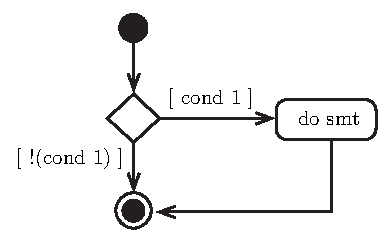
\includegraphics[width=0.50\linewidth]{01_Basics/figures/uml/SelectionStatement-00-UML-if-else.pdf}
\caption{UML \texttt{if-else} Activity Diagram Representation}
\label{fig:ch01_Basics_UML_SelStatement-00-if-else}
%~\ref{fig:ch01_Basics_UML_SelStatement-00-if-else} 
\end{figure}       %%%%%%%%%%%%%%%%%%%%%%% End Figure

\subsection{Iteration statement}
\subsubsection{\texttt{while}}
\begin{figure}[!h] %%%%%%%%%%%%%%%%%%%%%%% Begin Figure Directory
\centering
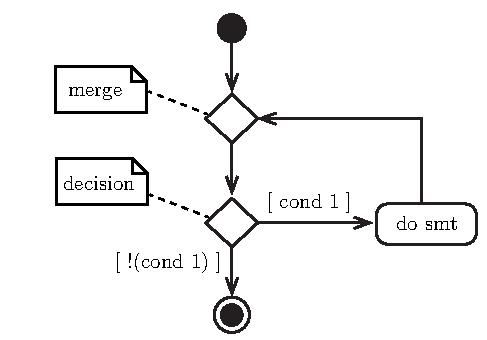
\includegraphics[width=0.50\linewidth]{01_Basics/figures/uml/IterationStatement-00-UML-while.pdf}
\caption{UML \texttt{if-else} Activity Diagram Representation}
\label{fig:ch01_Basics_UML_IterationStatement-00-while}
%~\ref{fig:ch01_Basics_UML_IterationStatement-00-while} 
\end{figure}       %%%%%%%%%%%%%%%%%%%%%%% End Figure



% no numbers listing
% \begin{lstlisting}[frame=tlrb,numbers=none,mathescape=true,escapechar=\%,columns=flexible]

% \begin{minipage}{.9\textwidth}
% \begin{lstlisting}[frame=tlrb,showlines=htrue,firstnumber=1,mathescape=true,escapechar=\%,columns=flexible]
% //code here
% \end{lstlisting}
% \end{minipage}

% \begin{lstlisting}[frame=tlrb,showlines=htrue,firstnumber=1,mathescape=true,escapechar=\%,columns=flexible]
% //Program 12.1
% \end{lstlisting}
    
%reference:
%~\ref{tab:t_ch11_UART_Registers} tab:t_ch12_edgeTriggeredModes
%~\ref{fig:RT_ch01} 
%\texttt{Ascii}
%\texttt{UART}
%\texttt{mailbox}
%\texttt{FIFO}
%\texttt{I/O}
%\underline{}
%$\texttt{b}_0$
%\sim = ~

%percent
%n%\%%10;

%for loops
% \newcounter{nnCount}
% \forloop{nnCount}{0}{\value{nnCount}<8}{&IME }  
% \forloop{nnCount}{0}{\value{nnCount}<8}{&PMC\arabic{nnCount} }


%Equation array
% \begin{eqnarray*}
%  & = & \text{minimun}\\
%  & = & \text{maximun}\\
%  & = &  \\
%  & = & \\
%  & = & 
% \end{eqnarray*}

% \begin{description}
% \item[Remark 1] If
% \end{description}

% \begin{description}
% \item[Remark 1] If
% \item[Remark 2] An
% \item[Remark 3] With 
% \end{description}

%Poner figura
% \begin{figure}[!h] %%%%%%%%%%%%%%%%%%%%%%% Begin Figure Directory
% \centering
% \includegraphics[width=0.70\linewidth]{figuresRT/ch06/RT-CH06-
% \caption{Free-space management.}
% \label{fig:ch01_00}
% %~\ref{ffig:ch01_00} 
% \end{figure}       %%%%%%%%%%%%%%%%%%%%%%% End Figure

%Poner Figura con minipages
% %begin minipages
% \begin{minipage}{.45\textwidth}
% %here some text.
% \end{minipage}
% \begin{minipage}{.55\textwidth}
% %and here the image.
% \centering
% \includegraphics[width=0.95\linewidth]{figures/ch12/ch12_lab12_squeme1.pdf}
% \captionof{figure}{Lab 12 diagram connections}
%\label{fig:RT_ch04_MACQ-EXAMPLE-01-oldDataIsLost}
%~\ref{fig:RT_ch04_MACQ-EXAMPLE-01-oldDataIsLost} 
% \end{minipage}
% \vspace{0.5cm}
% %end minipages


%\begin{enumerate}
%	\item Initialize timer and directions registers
%    \item Specify initial state
%    \item Perform FSM controller
%   \begin{enumerate}
%    	\item Call an output function, which depends on the state
%        \item Delay, which depends on the state
%        \item Call an input function to get the status of the coin sensors
%        \item Change states, which dependes on the state and the input
%    \end{enumerate}
%\end{enumerate}

% \begin{enumerate}
% 	\item Current instruction is finished,
%     \item Eight registers are pushed on the stack,
%     \item LR is set to 0xFFFFFFF9,
%     \item IPSR is set to the interrupt number,
%     \item PC is loaded with the interrupt vector
% \end{enumerate}

% Itemize categoriza poniendo (.) en lugar de números
% \begin{itemize} 
% 	\item I
% 	\item I
% 	\item Y
% 	\item Y
% 	\item Y
% 	\item Y
% 	\item 
% \end{itemize}

% \begin{table}[!h]
% \centering
% \begin{tabular}{|l|l|l|} \hline
% $p$ & bit Field & Interrupt         \\\hline
% $3$ & \bitsRange[31]{29} & Interrupt [$4m+3$]  \\\hline
% $2$ & \bitsRange[23]{21} & Interrupt [$4m+2$]  \\\hline
% $1$ & \bitsRange[15]{13} & Interrupt [$4m+1$]  \\\hline
% $0$ & \bitsRange[7]{5} & Interrupt [$4m$]   \\\hline
% \end{tabular}
% \caption{pasteCaption}
% \label{tab:t_rt_ch04_}
% ~\ref{tab:t_rt_ch04_}
% \end{table}

% Insertar URL
%\url{https://www.osha.gov/Publications/laboratory/OSHAfactsheet-laboratory-safety-noise.pdf}\\

% \newcommand{\bitsRange}[2][50]{\texttt{{#1}-{#2}}}
% \newcommand{\CustomHex}[2][0000]{\texttt{0x{#1}.{#2}}}
% \newcommand{\GPIOPort}[1]{\texttt{GPIO\_PORT{#1}}}
% \newcommand{\GPIOPortR}[2][A]{\texttt{GPIO\_PORT{#1}\_{#2}\_R}}
% \newcommand{\GPIOPortHandler}[1]{\texttt{GPIO\_PORT{#1}\_Handler}}
% \newcommand{\HandlerISR}[1]{\texttt{#1\_Handler}}
% \newcommand{\IRQnr}[1]{\texttt{{#1}}}
% \newcommand{\NVICPRI}[1]{\texttt{NVIC\_PRI{#1}\_R}}
% \newcommand{\NVICEN}[1]{\texttt{NVIC\_EN{#1}\_R}}
% \newcommand{\NVICDIS}[1]{\texttt{NVIC\_DIS{#1}\_R}}
% \newcommand{\Ttimer}[2][A]{\texttt{Timer\_{#2}{#1}}}
% \newcommand{\xNrbit}[1]{$#1$-\texttt{bit}}
% \newcommand{\xNrbits}[1]{$#1$-\texttt{bits}}
% \newcommand{\camouflagegreenCellColor}{\cellcolor[rgb]{0.47, 0.53, 0.42}}
% \newcommand{\lavenderCellColor}{\cellcolor[rgb]{0.9, 0.9, 0.98}}
% \newcommand{\volties}[2][0]{$\si{{#1}\volt}_{#2}$}
% \newcommand{\volti}[1]{$\si{{#1}\volt}$}
% \newcommand{\voltiposi}[1]{$+\si{{#1}\volt}$}
% \newcommand{\voltinega}[1]{$-\si{{#1}\volt}$}
\newpage
\section{Usefull Libraries}
\label{sec:Libraries}
%~\cref{sec:Libraries}
\subsection{\texttt{<cmath>}}

%%%%%%%%%%%%%%%%%%%%%%%%%%%%%%%%%%% CMATH TABLE
\begin{table}[!h]
\centering
\arrayrulecolor{black}
\begin{tabular}{l|l|l|l|} 
\cline{2-4}
 & Function & Description & Example \\ 
\hhline{>{\TabelleArrayColorGray}->{\arrayrulecolor{black}}---|}
\TabelleRowColorGray  01 & \texttt{ceil(x)} 
                         & rounds $x$ to the smallest integer not less than $x$ 
                         & \begin{tabular}[c]{@{}>{\TabelleRowCellGray}l@{}}
                         \texttt{ceil(9.2)} $=10.0$\\
                         \texttt{ceil(-9.8)} $=-9.0$\end{tabular} \\
02  & \texttt{cos(x)}  
    & trigonometric cosine of $x$ ($x$ in radians)  
    & $\texttt{cos(0.0)}=1.0$ \\
\TabelleRowColorGray 03 & \texttt{exp(x)} 
                        &  exponential function $e^{x}$
                        &  $\texttt{exp(1.0)} = 2.718282$\\
04  & \texttt{fabs(x)} 
    &  absolute value of $x$ 
    &   \begin{tabular}[c]{@{}l@{}}
        $\texttt{fabs(5.1)}=5.1$\\
        $\texttt{fabs(0.0)}=0.0$\\
        $\texttt{fabs(-8.6)}=8.6$\end{tabular} \\
\TabelleRowColorGray 05 & \texttt{floor(x)}  
                        &  rounds $x$ to the largest integer not greater than $x$
                        &  \begin{tabular}[c]{@{}>{\TabelleRowCellGray}l@{}}
                         \texttt{floor(9.2)} $=9.0$\\
                         \texttt{floor(-9.8)} $=-10$\end{tabular} \\
06  & \texttt{fmod(x, y)} 
    & remainder of $x/y$ as a floating-point number  
    & $\texttt{fmod(2.6, 1.2)}=0.2$ \\
\TabelleRowColorGray 07 & \texttt{log(x)} 
                        &  natural logarithm of $x$ (base $e$)
                        &  $\texttt{log()2.718282}=1.0$\\
08  & \texttt{log10(x)} 
    &  logarithm of $x$ (base 10)
    &  \begin{tabular}[c]{@{}l@{}}
        $\texttt{log10(10.0)}=1.0$\\
        $\texttt{log10(100.0)}=2.0$\end{tabular} \\
\TabelleRowColorGray 09 & \texttt{pow(x, y)} 
                        &  $x$ raised to power $y$, i.e. $x^y$
                        &  $\texttt{pow(2.7)}=2^{7}=128$\\
10  & \texttt{sin(x)} 
    &  trigonometric sine of x (x in radians)
    &  $\texttt{sin(0.0)}=0$\\
\TabelleRowColorGray 11 & \texttt{sqrt(x)} 
                        &  square root of x (where $x>=0$)
                        &  $\texttt{sin(9.0)}=3.0$\\
12  & \texttt{tan(x)} 
    &  trigonometric tangent of $x$ ($x$ in radians)
    &  $\texttt{tan(0.0)}=0$\\
\hhline{>{\TabelleArrayColorGray}->{\arrayrulecolor{black}}---|}
\end{tabular}
\end{table}

%%%%%%%% END CMATH TABLE






% \newcommand{\lavenderCellColor}{\cellcolor[rgb]{0.9, 0.9, 0.98}}
% \newcommand{\TabelleRowColorGray}{\rowcolor[rgb]{0.812,0.812,0.812}}
% \newcommand{\TabelleArrayColorGray}{\arrayrulecolor[rgb]{0.812,0.812,0.812}}
% \newcommand{\TabelleRowCellGray}{\cellcolor[rgb]{0.812,0.812,0.812}}
%

% no numbers listing
% \begin{lstlisting}[frame=tlrb,numbers=none,mathescape=true,escapechar=\%,columns=flexible]

% \begin{minipage}{.9\textwidth}
% \begin{lstlisting}[frame=tlrb,showlines=htrue,firstnumber=1,mathescape=true,escapechar=\%,columns=flexible]
% //code here
% \end{lstlisting}
% \end{minipage}

% \begin{lstlisting}[frame=tlrb,showlines=htrue,firstnumber=1,mathescape=true,escapechar=\%,columns=flexible]
% //Program 12.1
% \end{lstlisting}
    
%reference:
%~\ref{tab:t_ch11_UART_Registers} tab:t_ch12_edgeTriggeredModes
%~\ref{fig:RT_ch01} 
%\texttt{Ascii}
%\texttt{UART}
%\texttt{mailbox}
%\texttt{FIFO}
%\texttt{I/O}
%\underline{}
%$\texttt{b}_0$
%\sim = ~

%percent
%n%\%%10;

%for loops
% \newcounter{nnCount}
% \forloop{nnCount}{0}{\value{nnCount}<8}{&IME }  
% \forloop{nnCount}{0}{\value{nnCount}<8}{&PMC\arabic{nnCount} }


%Equation array
% \begin{eqnarray*}
%  & = & \text{minimun}\\
%  & = & \text{maximun}\\
%  & = &  \\
%  & = & \\
%  & = & 
% \end{eqnarray*}

% \begin{description}
% \item[Remark 1] If
% \end{description}

% \begin{description}
% \item[Remark 1] If
% \item[Remark 2] An
% \item[Remark 3] With 
% \end{description}

%Poner figura
% \begin{figure}[!h] %%%%%%%%%%%%%%%%%%%%%%% Begin Figure Directory
% \centering
% \includegraphics[width=0.70\linewidth]{figuresRT/ch06/RT-CH06-
% \caption{Free-space management.}
% \label{fig:ch01_00}
% %~\ref{ffig:ch01_00} 
% \end{figure}       %%%%%%%%%%%%%%%%%%%%%%% End Figure

%Poner Figura con minipages
% %begin minipages
% \begin{minipage}{.45\textwidth}
% %here some text.
% \end{minipage}
% \begin{minipage}{.55\textwidth}
% %and here the image.
% \centering
% \includegraphics[width=0.95\linewidth]{figures/ch12/ch12_lab12_squeme1.pdf}
% \captionof{figure}{Lab 12 diagram connections}
%\label{fig:RT_ch04_MACQ-EXAMPLE-01-oldDataIsLost}
%~\ref{fig:RT_ch04_MACQ-EXAMPLE-01-oldDataIsLost} 
% \end{minipage}
% \vspace{0.5cm}
% %end minipages

% %Poner Figura y al costado codigo
% %begin minipages
% \begin{minipage}{.60\textwidth}
% %%%%%%%%%%%%%%%%%%%%%%%%%%%%%%%%%Figure Selection Statement - while
% \centering
% 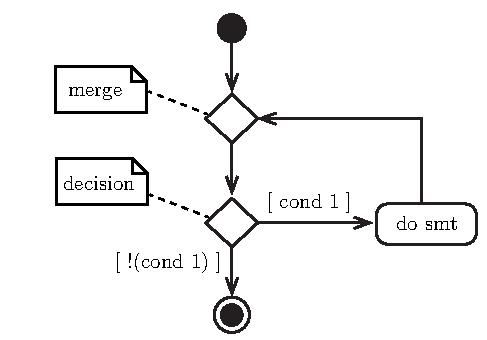
\includegraphics[width=0.50\linewidth]{01_Basics/figures/uml/IterationStatement-00-UML-while.pdf}
% \captionof{figure}{UML \texttt{while} Activity Diagram Representation}
% \label{fig:ch01_Basics_UML_IterationStatement-00-while}
% %~\ref{fig:ch01_Basics_UML_IterationStatement-00-while} 
% %%%%%%%%%%%%%%%%%%%%%%%%%%End figure
% \end{minipage}
% \begin{minipage}{.25\textwidth}
% %%%%%%%%%%%%%%%%%%%%%%%%%%%%%%%%%Begin code
% \begin{lstlisting}[frame=tlrb,numbers=none,mathescape=true,escapechar=\%,columns=flexible]
% some awesome code here
% \end{lstlisting}
% %%%%%%%%%%%%%%%%%%End Code
% \end{minipage}
% \vspace{0.5cm}
% %end minipages


%\begin{enumerate}
%	\item Initialize timer and directions registers
%    \item Specify initial state
%    \item Perform FSM controller
%   \begin{enumerate}
%    	\item Call an output function, which depends on the state
%        \item Delay, which depends on the state
%        \item Call an input function to get the status of the coin sensors
%        \item Change states, which dependes on the state and the input
%    \end{enumerate}
%\end{enumerate}

% \begin{enumerate}
% 	\item Current instruction is finished,
%     \item Eight registers are pushed on the stack,
%     \item LR is set to 0xFFFFFFF9,
%     \item IPSR is set to the interrupt number,
%     \item PC is loaded with the interrupt vector
% \end{enumerate}

% Itemize categoriza poniendo (.) en lugar de números
% \begin{itemize} 
% 	\item I
% 	\item I
% 	\item Y
% 	\item Y
% 	\item Y
% 	\item Y
% 	\item 
% \end{itemize}

% \begin{table}[!h]
% \centering
% \begin{tabular}{|l|l|l|} \hline
% $p$ & bit Field & Interrupt         \\\hline
% $3$ & \bitsRange[31]{29} & Interrupt [$4m+3$]  \\\hline
% $2$ & \bitsRange[23]{21} & Interrupt [$4m+2$]  \\\hline
% $1$ & \bitsRange[15]{13} & Interrupt [$4m+1$]  \\\hline
% $0$ & \bitsRange[7]{5} & Interrupt [$4m$]   \\\hline
% \end{tabular}
% \caption{pasteCaption}
% \label{tab:t_rt_ch04_}
% ~\ref{tab:t_rt_ch04_}
% \end{table}

% Insertar URL
%\url{https://www.osha.gov/Publications/laboratory/OSHAfactsheet-laboratory-safety-noise.pdf}\\

% \newcommand{\bitsRange}[2][50]{\texttt{{#1}-{#2}}}
% \newcommand{\CustomHex}[2][0000]{\texttt{0x{#1}.{#2}}}
% \newcommand{\GPIOPort}[1]{\texttt{GPIO\_PORT{#1}}}
% \newcommand{\GPIOPortR}[2][A]{\texttt{GPIO\_PORT{#1}\_{#2}\_R}}
% \newcommand{\GPIOPortHandler}[1]{\texttt{GPIO\_PORT{#1}\_Handler}}
% \newcommand{\HandlerISR}[1]{\texttt{#1\_Handler}}
% \newcommand{\IRQnr}[1]{\texttt{{#1}}}
% \newcommand{\NVICPRI}[1]{\texttt{NVIC\_PRI{#1}\_R}}
% \newcommand{\NVICEN}[1]{\texttt{NVIC\_EN{#1}\_R}}
% \newcommand{\NVICDIS}[1]{\texttt{NVIC\_DIS{#1}\_R}}
% \newcommand{\Ttimer}[2][A]{\texttt{Timer\_{#2}{#1}}}
% \newcommand{\xNrbit}[1]{$#1$-\texttt{bit}}
% \newcommand{\xNrbits}[1]{$#1$-\texttt{bits}}
% \newcommand{\camouflagegreenCellColor}{\cellcolor[rgb]{0.47, 0.53, 0.42}}
% \newcommand{\lavenderCellColor}{\cellcolor[rgb]{0.9, 0.9, 0.98}}
% \newcommand{\volties}[2][0]{$\si{{#1}\volt}_{#2}$}
% \newcommand{\volti}[1]{$\si{{#1}\volt}$}
% \newcommand{\voltiposi}[1]{$+\si{{#1}\volt}$}
% \newcommand{\voltinega}[1]{$-\si{{#1}\volt}$}
\newpage
\section{Arrays and Vectors}
\label{sec:Arrays-and-Vectors}
%~\cref{sec:Libraries}
\subsection{Difference}
\begin{itemize}
    \item \CppKeywordSpecial{array} - they are fixed-size collections consisting of data items of the same type
    \item \CppKeywordSpecial{vector} - same as array but they can grow and shrink dynamically at execution time. 
\end{itemize}

\subsection{Remarks}
\begin{itemize}
    \item When speaking about the elements of an array you could say:
\end{itemize}
\begin{table}[!h]
\centering
\begin{tblr}{
  row{3} = {c},
  row{4} = {c},
  cell{1}{1} = {c=3}{},
  cell{2}{1} = {c},
  cell{3}{1} = {r},
  cell{4}{1} = {r},
  hlines,
  vlines,
}
Example with an arrray declared as \texttt{arr}&  & \\
 & Refer to Subscript & Actual element in the array\\
"sevent element of the array" & \texttt{arr[6]} & 7\\
"array element 7"             & \texttt{arr[7]} & 8
\end{tblr}
\end{table}
\begin{itemize}
    \item Remeber \CppKeywordCommon{size\_t} := unsigned integral type. For more info see Section~\ref{subsec:Data-Type-Size-t}
\end{itemize}


\subsection{Array declaration}
%%%%%%%%%%%%%%%%%%%%%%%%%%%%%%%%%%%%%%%%%%%%%%%% Array Declaration
%\begin{minipage}{\MPWxCONSIDERxNUMERATIONxFORxLISTING\textwidth}
%\end{minipage}{\hspaceNumerationBeforeListing}
\begin{minipage}{\MPWxLARGExLISTING\textwidth} % = 0.8 times \textwidth
\vspaceTextToListing % =\vspace{0.1cm}
\begin{CPPCode}
array<type, arraySize> arrayName;
\end{CPPCode}
\end{minipage}
%%%%%%%%%%%%%%%%%%%%%%%% END Array Declaration
\\
Examples:\\
%%%%%%%%%%%%%%%%%%%%%%%%%%%%%%%%%%%%%%%%%%%%%%%% Array Declaration Examples
\begin{minipage}{\MPWxLARGExLISTING\textwidth} % = 0.8 times \textwidth
\vspaceTextToListing % =\vspace{0.1cm}
\begin{CPPCode}
array<int, 12> n1; ¿\hspace{3.2cm}¿// n1 is an array of 5 int values

array<int, 5> n2{32, 27, 64, 18, 95}; // ¿\codecomment{declaration and init}¿

array<int, 5> n3{}; ¿\hspace{3.0cm}¿// ¿\codecomment{initialize elements with 0}¿

//constant varaiable can be used to specify ¿\codecomment{array size}¿
const size_t arraySize{5} 
array<int, ¿arraySize¿> n4{10, 20, 30}; //values; 
\end{CPPCode}
\end{minipage}
\\
%%%%%%%%%%%%%%%%%%%%%%%% END Array Declaration examples
If there are fewer initializers than array elements, the remaining array elements are initialized
to zero.\\

\noindent Going through an array called \texttt{a}\\
%%%%%%%%%%%%%%%%%%%%%%%%%%%%%%%%%%%%%%%%%%%%%%%%% going through array
\begin{minipage}{\MPWxLARGExLISTING\textwidth} % = 0.8 times \textwidth
\vspaceTextToListing % =\vspace{0.1cm}
\begin{CPPCode}
for (size_t j{0}; j ¿<¿ a.size(); ++j)
{
    //¿\codecomment{do smt}¿
}
\end{CPPCode}
\end{minipage}
%%%%%%%%%%%%%%%%%%%%%%%% END going through array

\subsection{Array Declaration in range-Based style}
%%%%%%%%%%%%%%%%%%%%%%%%%%%%%%%%%%%%%%%%%%%%%%%%% 
\begin{minipage}{\MPWxXSSxLISTING\textwidth} % = 0.36 times \textwidth
\vspace{-0.35cm}
\vspaceTextToListing % =\vspace{0.1cm}
\begin{CPPCode}
//Range-based style
array<int, 5> items{1, 2, 3, 4, 5};
for (int item : items)
{
    cout ¿<¿¿<¿ item ¿<¿¿<¿ " ";
}
\end{CPPCode}
\end{minipage}
\hspaceListingToListing
\begin{minipage}{\MPWxXSxLISTING\textwidth} % = 0.8 times \textwidth
\vspaceTextToListing % =\vspace{0.1cm}
\begin{CPPCode}
//Equivalent to:
for ( int counter{0}; 
             counter ¿<¿ items.size(); 
          ++counter )
{
    cout ¿<¿¿<¿ items[counter] ¿<¿¿<¿ " ";
}
\end{CPPCode}
\end{minipage}
\\
%%%
\noindent To modify the elements we need the ampersand symbol \texttt{\&}, i.e.:\\
%%%%%%%%%%%%%%%%%%%%%%%%%%%%%%%%%%%%%%%%%%%%%%%%% 
\begin{minipage}{\MPWxLARGExLISTING\textwidth} % = 0.8 times \textwidth
\vspaceTextToListing % =\vspace{0.1cm}
\begin{CPPCode}
for (int& itemRef : items)
{
    itemRef *= 2;    // ¿\codecomment{do smt modifying the content}¿
}
\end{CPPCode}
\end{minipage}

\subsection{Multidimensional array}
\begin{minipage}{\MPWxSMALLxLISTING\textwidth} % = 0.8 times \textwidth
\vspaceTextToListing % =\vspace{0.1cm}
\begin{CPPCode}
#include <iostream>
#include <array>
/* GLOBALS VARIABLES*/
const size_t rows{2};
const size_t columns{3};

/* PROTOTYPES */
void printArray(const array<array<int, columns>, rows>&);
\end{CPPCode}
\end{minipage}
\hspaceListingToListing
\begin{minipage}{\MPWxXXSxLISTING\textwidth} % = 0.8 times \textwidth
Note that \CppKeywordCommon{const} is used in the function prototype since we are not changing the values. Meanwhile \CppKeywordCommon{const}\texttt{\&} in the row's declaration indicates that the reference \textbf{cannot} be used to \textbf{modify} the rows and prevents each row from being copied into the range variable.
\end{minipage}
\\
\begin{minipage}{\MPWxSMALLxLISTING\textwidth} % = 0.8 times \textwidth
\vspaceTextToListing % =\vspace{0.1cm}
\begin{CPPCode}
int main()
{
    array<array<int, columns>, rows> array1{1, 2, 3, 4, 5, 6};
    array<array<int, columns>, rows> array2{1, 2, 3, 4, 5};

    cout ¿<¿¿<¿ "Values ¿in¿ array1 by row are:" ¿<¿¿<¿ endl;
    printArray(array1);

    cout ¿<¿¿<¿ "\nValues ¿in¿ array2 by row are:" ¿<¿¿<¿ endl;
    printArray(array2);
}

void printArray(const array<array<int, columns>, rows>& a)
{
    for (auto const& row : a)
    {
        for (auto const& element : row)
        {
            cout ¿<¿¿<¿ element ¿<¿¿<¿ ' ';            
        }

        cout ¿<¿¿<¿ endl;
    }
}
\end{CPPCode}
\end{minipage}
\hspaceListingToListing
\begin{minipage}{\MPWxXXSxLISTING\textwidth} % = 0.8 times \textwidth
\vspace{5cm}
\vspaceTextToListing % =\vspace{0.1cm}
\begin{Terminal}
OUTPUT:
-----------------------------
Values in array1 by row are:
1 2 3
4 5 6

Values in array2 by row are:
1 2 3
4 5 0
\end{Terminal}
\end{minipage}\\
As an example, the next Listing present the multidimensional nested counter-controlled statement\\
\begin{minipage}{\MPWxSMALLxLISTING\textwidth} % = 0.8 times \textwidth
\vspaceTextToListing % =\vspace{0.1cm}
\begin{CPPCode}
for (size_t row{0}; row ¿<¿ a.size(); ++row)
{
    for (size_t column{0}; column ¿<¿ a[row].size(); ++column) 
    {
        cout ¿<¿¿<¿ a[row][column] ¿<¿¿<¿ ' ';
    }
    
    cout ¿<¿¿<¿ endl;
}
\end{CPPCode}
\end{minipage}

\subsection{Local Arrays}
A static local variable in a function definition exists for the program’s duration but is visible only in the function’s body.
\subsubsection{\CppKeywordCommon{static} local Array}
By declaring a local array as \CppKeywordCommon{static}, then it is not created and initialized each time the program calls the function and is not destroyed each time the function terminates. This can improve performance especially when using large arrays~\cite{deitel2017c++}.\\

\noindent If a static array is not initialized explicitly by you, \textbf{each element of that array is initialized to zero by the compiler} when the array is created. Recall that C++ does not perform such default initialization for other local variables.\\
\noindent
\begin{minipage}{\MPWxXSxLISTING\textwidth} % = 0.7 times \textwidth
\vspaceTextToListing % =\vspace{0.1cm}
        \begin{CPPCode}
const size_t arraySize{3};
void SomeFunction(void)
{
    // Local ¿\codecomment{array}¿
    array<int, arraySize> arr{1, 2, 3}
}
        \end{CPPCode}
    \end{minipage}
    \hspaceListingXSToListingXS
    \begin{minipage}{\MPWxSxLISTING\textwidth} % = 0.7 times \textwidth
    \vspaceTextToListing
        \begin{CPPCode}
const size_t arraySize{3};
void SomeFunction(void)
{
        // Static local ¿\codecomment{array}¿
    static array<int, arraySize> arrAsStaticLocal
}
        \end{CPPCode}
\end{minipage}

\subsection{Built-In Arrays}
\label{subsec:Built-In-Arrays}
%~\cref{subsec:Built-In-Arrays}
It is a fixed-size data structure. The compiler reserves the appropiate amount of memory. Its declaration goes as follows:
\codeLine{type arrayName[arraySize]}\\
where \CppCommonCode{arraySize}$>0$ and must be integer constant.\\
\begin{minipage}{\MPWxXSxLISTING\textwidth} % = 0.7 times \textwidth
\vspaceTextToListing % =\vspace{0.1cm}
        \begin{CPPCode}
//init opt 01
int n[5]{50, 20, 30, 10, 40}
        \end{CPPCode}
    \end{minipage}
    \hspaceListingXSToListingXS
    \begin{minipage}{\MPWxSxLISTING\textwidth} % = 0.7 times \textwidth
    \vspaceTextToListing
        \begin{CPPCode}
//init opt 02  - possible but not recommended
int n[]{50, 20, 30, 10, 40} //arrSize no specified.
        \end{CPPCode}
\end{minipage}
\begin{itemize}
    \item if you provide fewer initializers than number of elements, the remaining elements are value initialized, i.e.
    \begin{itemize}
        \item numeric types to $0$, 
        \item \CppCommonCode{bool}s to false,
        \item \textbf{pointers} to \CppCommonCode{nullptr} (Pointers are explained in Section~\ref{sec:Pointers}) and 
        \item class objects to its default constructor.
    \end{itemize}

    \item built-in arrays don't know their own size, so a function that processes a built-in array should also have a parameter to receive its size.

    \item The compiler does not distinguish between a function that receives a pointer and a function that receives a built in array. I.e. each time that the compiler finds a built-in array notation it converts to pointer  notation.\\
    \begin{minipage}{\MPWxXXSxLISTING\textwidth} % = 0.7 times \textwidth
\vspaceTextToListing % =\vspace{0.1cm}
        \begin{CPPCode}
// Built-in Array notation
foo(const int values[])
        \end{CPPCode}
    \end{minipage}
    \hspaceListingXSToListingXS
    \begin{minipage}{\MPWxXSxLISTING\textwidth} % = 0.7 times \textwidth
    \vspaceTextToListing
        \begin{CPPCode}
// Pointer notation
foo(const int* values)
        \end{CPPCode}
\end{minipage}
    \item Note that \CppCommonCode{const int* values} is read as "values is a pointer to a integer constant".
\end{itemize}

\subsection{Examples}

\begin{minipage}{\MPWxLARGExLISTING\textwidth} % = 0.8 times \textwidth
\vspaceTextToListing % =\vspace{0.1cm}
\begin{CPPCode}
//example printArray
// output ¿\codecomment{array with two rows and three columns}¿
void printArray(const array<array<int, columns>, row>& row_x)
{
    // loop through ¿\codecomment{array}'¿s rows
    for (auto const& row : row_x)
    {
        // loop through columns of current row
        for (auto const& col : row)
        {
            cout ¿<¿¿<¿ element ¿<¿¿<¿ ' ';
        }
    }
}
\end{CPPCode}
\end{minipage}
\\
which is equivalent to:\\
\begin{minipage}{\MPWxLARGExLISTING\textwidth} % = 0.8 times \textwidth
\vspaceTextToListing % =\vspace{0.1cm}
\begin{CPPCode}
for (size_t row{0}; row ¿<¿ a.size(); ++row) 
{
    for (size_t column{0}; column ¿<¿ a[row].size(); ++column)
    {
        cout ¿<¿¿<¿ a[row][column] ¿<¿¿<¿ ' ';
    }
    cout ¿<¿¿<¿ endl;
}
\end{CPPCode}
\end{minipage}
\\

%%%%%%%%%%%%%%%%%%%%%%%% END going through array
% no numbers listing
% \begin{lstlisting}[frame=tlrb,numbers=none,mathescape=true,escapechar=\%,columns=flexible]

% \begin{minipage}{.9\textwidth}
% \begin{lstlisting}[frame=tlrb,showlines=htrue,firstnumber=1,mathescape=true,escapechar=\%,columns=flexible]
% //code here
% \end{lstlisting}
% \end{minipage}

% \begin{lstlisting}[frame=tlrb,showlines=htrue,firstnumber=1,mathescape=true,escapechar=\%,columns=flexible]
% //Program 12.1
% \end{lstlisting}
    
%reference:
%~\ref{tab:t_ch11_UART_Registers} tab:t_ch12_edgeTriggeredModes
%~\ref{fig:RT_ch01} 
%\texttt{Ascii}
%\texttt{UART}
%\texttt{mailbox}
%\texttt{FIFO}
%\texttt{I/O}
%\underline{}
%$\texttt{b}_0$
%\sim = ~

%percent
%n%\%%10;

%for loops
% \newcounter{nnCount}
% \forloop{nnCount}{0}{\value{nnCount}<8}{&IME }  
% \forloop{nnCount}{0}{\value{nnCount}<8}{&PMC\arabic{nnCount} }


%Equation array
% \begin{eqnarray*}
%  & = & \text{minimun}\\
%  & = & \text{maximun}\\
%  & = &  \\
%  & = & \\
%  & = & 
% \end{eqnarray*}

% \begin{description}
% \item[Remark 1] If
% \end{description}

% \begin{description}
% \item[Remark 1] If
% \item[Remark 2] An
% \item[Remark 3] With 
% \end{description}

%Poner figura
% \begin{figure}[!h] %%%%%%%%%%%%%%%%%%%%%%% Begin Figure Directory
% \centering
% \includegraphics[width=0.70\linewidth]{figuresRT/ch06/RT-CH06-
% \caption{Free-space management.}
% \label{fig:ch01_00}
% %~\ref{ffig:ch01_00} 
% \end{figure}       %%%%%%%%%%%%%%%%%%%%%%% End Figure

%Poner Figura con minipages
% %begin minipages
% \begin{minipage}{.45\textwidth}
% %here some text.
% \end{minipage}
% \begin{minipage}{.55\textwidth}
% %and here the image.
% \centering
% \includegraphics[width=0.95\linewidth]{figures/ch12/ch12_lab12_squeme1.pdf}
% \captionof{figure}{Lab 12 diagram connections}
%\label{fig:RT_ch04_MACQ-EXAMPLE-01-oldDataIsLost}
%~\ref{fig:RT_ch04_MACQ-EXAMPLE-01-oldDataIsLost} 
% \end{minipage}
% \vspace{0.5cm}
% %end minipages

% %Poner Figura y al costado codigo
% %begin minipages
% \begin{minipage}{.60\textwidth}
% %%%%%%%%%%%%%%%%%%%%%%%%%%%%%%%%%Figure Selection Statement - while
% \centering
% 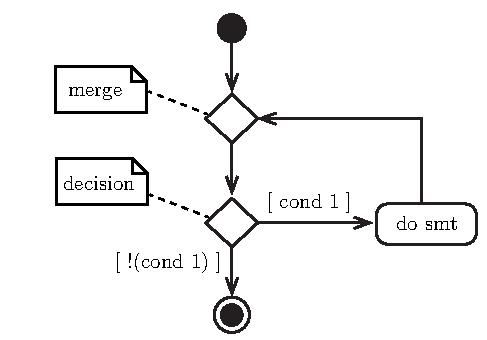
\includegraphics[width=0.50\linewidth]{01_Basics/figures/uml/IterationStatement-00-UML-while.pdf}
% \captionof{figure}{UML \texttt{while} Activity Diagram Representation}
% \label{fig:ch01_Basics_UML_IterationStatement-00-while}
% %~\ref{fig:ch01_Basics_UML_IterationStatement-00-while} 
% %%%%%%%%%%%%%%%%%%%%%%%%%%End figure
% \end{minipage}
% \begin{minipage}{.25\textwidth}
% %%%%%%%%%%%%%%%%%%%%%%%%%%%%%%%%%Begin code
% \begin{lstlisting}[frame=tlrb,numbers=none,mathescape=true,escapechar=\%,columns=flexible]
% some awesome code here
% \end{lstlisting}
% %%%%%%%%%%%%%%%%%%End Code
% \end{minipage}
% \vspace{0.5cm}
% %end minipages


%\begin{enumerate}
%	\item Initialize timer and directions registers
%    \item Specify initial state
%    \item Perform FSM controller
%   \begin{enumerate}
%    	\item Call an output function, which depends on the state
%        \item Delay, which depends on the state
%        \item Call an input function to get the status of the coin sensors
%        \item Change states, which dependes on the state and the input
%    \end{enumerate}
%\end{enumerate}

% \begin{enumerate}
% 	\item Current instruction is finished,
%     \item Eight registers are pushed on the stack,
%     \item LR is set to 0xFFFFFFF9,
%     \item IPSR is set to the interrupt number,
%     \item PC is loaded with the interrupt vector
% \end{enumerate}

% Itemize categoriza poniendo (.) en lugar de números
% \begin{itemize} 
% 	\item I
% 	\item I
% 	\item Y
% 	\item Y
% 	\item Y
% 	\item Y
% 	\item 
% \end{itemize}

% \begin{table}[!h]
% \centering
% \begin{tabular}{|l|l|l|} \hline
% $p$ & bit Field & Interrupt         \\\hline
% $3$ & \bitsRange[31]{29} & Interrupt [$4m+3$]  \\\hline
% $2$ & \bitsRange[23]{21} & Interrupt [$4m+2$]  \\\hline
% $1$ & \bitsRange[15]{13} & Interrupt [$4m+1$]  \\\hline
% $0$ & \bitsRange[7]{5} & Interrupt [$4m$]   \\\hline
% \end{tabular}
% \caption{pasteCaption}
% \label{tab:t_rt_ch04_}
% ~\ref{tab:t_rt_ch04_}
% \end{table}

% Insertar URL
%\url{https://www.osha.gov/Publications/laboratory/OSHAfactsheet-laboratory-safety-noise.pdf}\\

% \newcommand{\bitsRange}[2][50]{\texttt{{#1}-{#2}}}
% \newcommand{\CustomHex}[2][0000]{\texttt{0x{#1}.{#2}}}
% \newcommand{\GPIOPort}[1]{\texttt{GPIO\_PORT{#1}}}
% \newcommand{\GPIOPortR}[2][A]{\texttt{GPIO\_PORT{#1}\_{#2}\_R}}
% \newcommand{\GPIOPortHandler}[1]{\texttt{GPIO\_PORT{#1}\_Handler}}
% \newcommand{\HandlerISR}[1]{\texttt{#1\_Handler}}
% \newcommand{\IRQnr}[1]{\texttt{{#1}}}
% \newcommand{\NVICPRI}[1]{\texttt{NVIC\_PRI{#1}\_R}}
% \newcommand{\NVICEN}[1]{\texttt{NVIC\_EN{#1}\_R}}
% \newcommand{\NVICDIS}[1]{\texttt{NVIC\_DIS{#1}\_R}}
% \newcommand{\Ttimer}[2][A]{\texttt{Timer\_{#2}{#1}}}
% \newcommand{\xNrbit}[1]{$#1$-\texttt{bit}}
% \newcommand{\xNrbits}[1]{$#1$-\texttt{bits}}
% \newcommand{\camouflagegreenCellColor}{\cellcolor[rgb]{0.47, 0.53, 0.42}}
% \newcommand{\lavenderCellColor}{\cellcolor[rgb]{0.9, 0.9, 0.98}}
% \newcommand{\volties}[2][0]{$\si{{#1}\volt}_{#2}$}
% \newcommand{\volti}[1]{$\si{{#1}\volt}$}
% \newcommand{\voltiposi}[1]{$+\si{{#1}\volt}$}
% \newcommand{\voltinega}[1]{$-\si{{#1}\volt}$}



%new page before acronyms
\newpage
%chapter*{\glossarytitlename}
\addcontentsline{toc}{chapter}{Abbreviations}
\begin{acronym}[ABCDEFGHIJK]
%A
\acro{API}{Application Programming Interface} %\ac{API}
\acro{APB}{Advanced Peripheral Bus} %\ac{APB}
%D
\acro{DAE}{Differential-Algebraic Equation}
\acro{DDI}{Differential Dissipativity Inequality}%\ac{DDI} 
\acro{DOF}{Degrees of Freedom}
%E
\acro{ES}{Energy Shaping}
%I
\acro{ISR}{Interrupt Service Routine} %\ac{ISR}
%P
\acro{PBC}{Passivity Based Control}
\acro{PDE}{Partial Differential Equation}
\acro{PFL}{Partial Feedback Linearization}
\acro{pH}{port-Hamiltonian}
%R
\acro{RTOS}{Real Time Operating System} %\ac{RTOS}
%S
\acro{SMC}{Sliding Mode Control}
\acro{SysML}{System Modelling Language} % \ac{UMS}
%U
\acro{UMS}{Underactuated Mechanical System} % \ac{UMS}
\acro{UML}{Unified Modelling Language} % \ac{UMS}
%Z

\end{acronym}
\clearpage

\bibliographystyle{IEEEtran}
\bibliography{myReferences}
\end{document}
